\chapter{Temporal Coherence}
\label{chap:markovnet}

In this chapter, we consider methods for exploiting temporal correlation between CSI of subsequent timeslots. The \emph{coherence time} of a channel is the amount of time that a channel estimate can be used before that estimate's SNR falls beneath a given threshold \cite{ref:Chopra2016ChannelAging}. Within this window of time ($\Delta t = t_i - t_{i-1}$), the correlation between CSI matrices $\mathbf H_{i}$ and $\mathbf H_{i-1}$ is high (see Figure~\ref{fig:csi_img_gt} for an illustrative example). 
% Works exploiting temporal coherence use CSI matrices from previous timeslots to supplement subsequent estimates \cite{ref:Wang2019CsiNetLSTM}.

\begin{figure}[htb] \centering 
  % 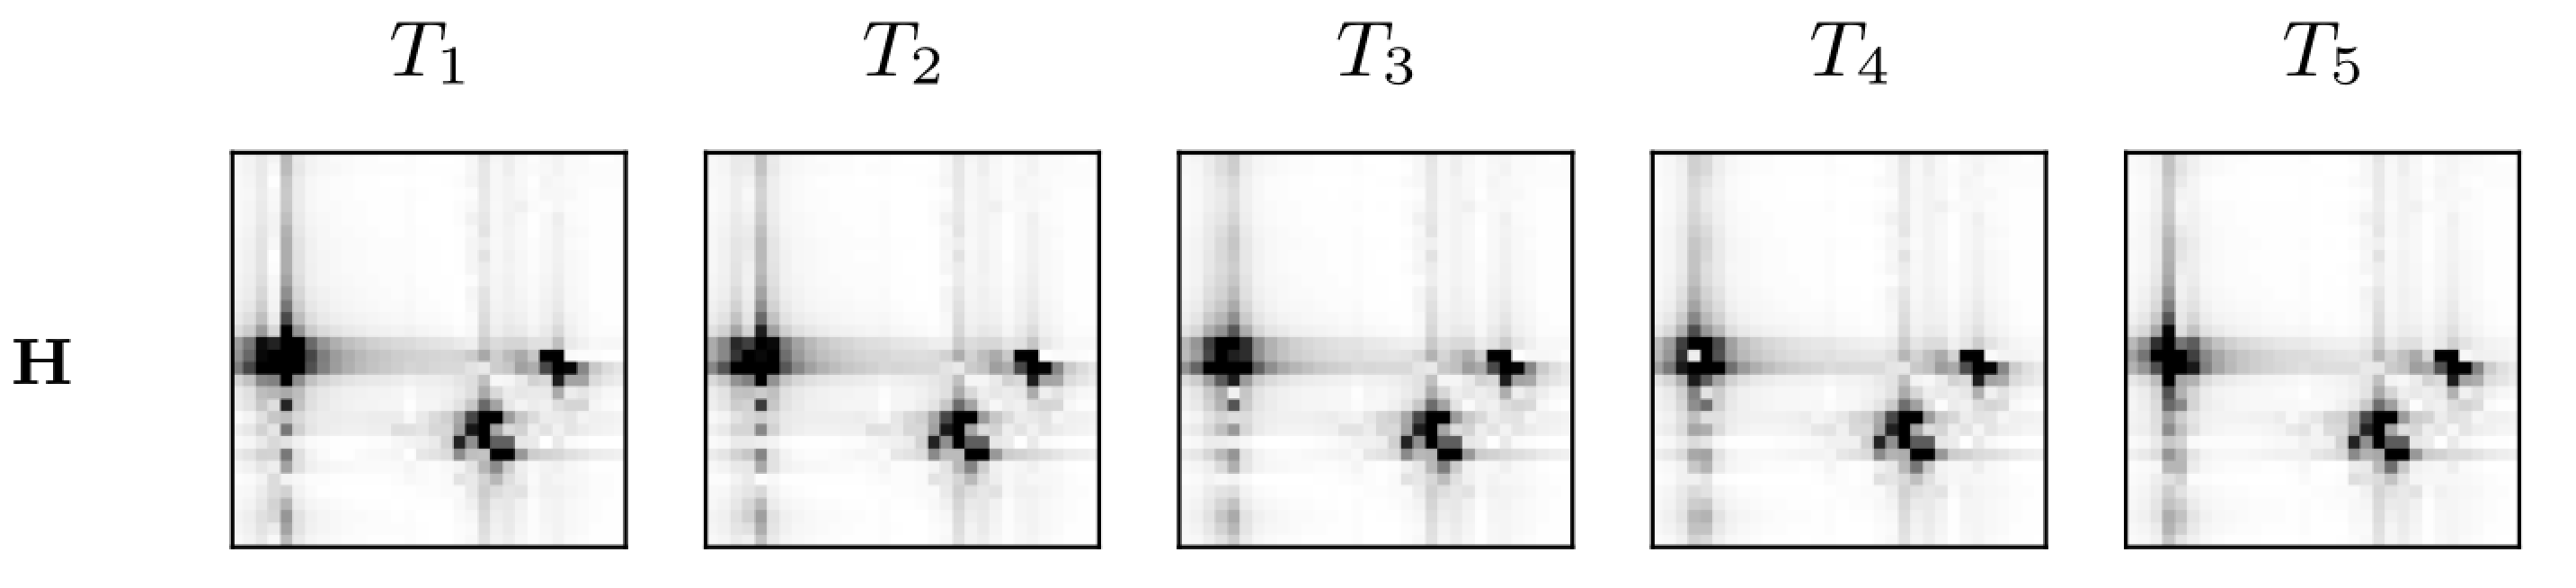
\includegraphics[width=0.9\linewidth]{batch0_csi_gt.png}
{
  \fontsize{10pt}{12pt}
  \def\svgwidth{1.0\columnwidth}
  \input{images/batch0_csi_gt.pdf_tex}
}
  \caption{Ground truth CSI ($\mathbf H$) for five timeslots ($t_1$ through $t_5$) on one sample from the validation set of the outdoor dataset.} 
  \label{fig:csi_img_gt} 
\end{figure}

% Other works in channel state estimation exploit temporal coherence.

Assuming the channel exhibits temporal coherence within a certain window of time,
a reasonably accurate CSI estimate at time $t_{i-1}$ can be used to estimate the CSI at time $t_i$.
Generically, we can write this estimator as
\begin{align}
\grave{\mathbf H}_i &= h(\hat{\mathbf H}_{i-1}) \label{eq:gen_estim}
\end{align}
where $\mathbf{H}_i$ is the CSI matrix at time $t_i$ and $\hat{\mathbf H}_i$ is its estimator. 
The estimation error under $\grave{\mathbf H}_i$ is
\begin{align}
\mathbf E_{i} &= \mathbf H_{i} - \grave{\mathbf H}_{i}. \label{eq:diff_err}
\end{align}

\section{Recurrent Neural Networks}

Prior work in temporal correlation for CSI estimation utilized state-space methods such as the Kalman filter \cite{ref:Huber2006improved,ref:Ali2020BayesKalmanFilter,ref:Kim2021KalmanVsML}. Since it relies on explicit state space and noise models, the Kalman filter's predictive power in CSI estimation is limited. Furthermore, such work generally does not propose a method for feedback compression, making comparison with the following ML methods difficult.

Recent works have leveraged recurrent neural networks (RNNs) to exploit temporal correlation for CSI estimation \cite{ref:Lu2019RecCsiNet, ref:Liao2019BiLSTM, ref:Li2020SpatTempLSTM,
 ref:Jang2019Delay,ref:Wang2019CsiNetLSTM}. RNNs include recurrent layers, such as the long short-term memory (LSTM) cell or the gated recurrent unit (GRU), which are capable of learning long-term dependencies of a given process through backpropagation \cite{ref:Hermans2013Training} and can be used to predict future states of the process \cite{ref:Pascanu2014HowTo}.

\begin{figure}[htb]
	\centering
	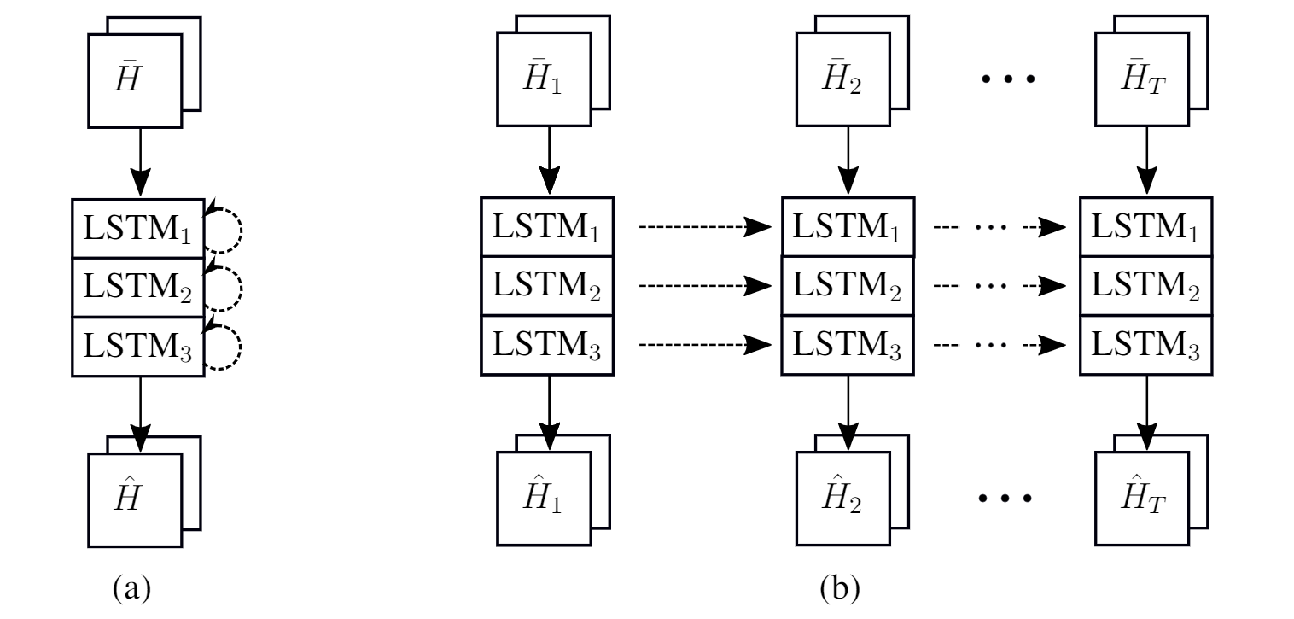
\includegraphics[width=.9\textwidth]{lstm-example-unroll.pdf}
	\medskip
	\caption{An example of LSTMs used for CSI estimation. (a) ``Stacked'' LSTM network of depth 3 shown with recurrent connections. (b) Same LSTM network ``unrolled" into $T$ timeslots }
	\label{fig:lstm_example}
\end{figure}

RNNs have been used extensively in natural language processing (NLP) for machine translation \cite{ref:Sutskever2014seq2seq} and sentiment extraction \cite{ref:Irsoy2014opinion}. For such works in NLP, authors have empirically found ``stacked'' or ``deep'' RNNs to be effective (e.g., Fig.~\ref{fig:lstm_example}), hypothesizing that having multiple recurrent layers allows the network to extract different semantic timescales \cite{ref:Irsoy2014opinion, ref:Bengio2009Learning}. Works in CSI estimation have taken cues from this work in NLP, proposing CSI estimation networks with stacked LSTMs after a sequence of autoencoders \cite{ref:Wang2019CsiNetLSTM}. While such work has demonstrated the utility of RNNs, the computational cost of LSTMs can be prohibitively high. For example, the RNN portion of the network proposed in \cite{ref:Wang2019CsiNetLSTM} accounts for $10^8$ additional parameters. Since channel estimation should not place an undue computational burden on the communications system, LSTMs can be problematic.

\section{Differential Encoding}

Rather than use RNNs to extract temporal dependencies in CSI data, we proposed a lightweight network based on the principle of differential encoding. We trained a network to estimate the error (\ref{eq:diff_err}) under a linear estimator, 
\begin{align*}
	\grave{\mathbf H}_i &=  \hat{\mathbf H}_{i-1} \mathbf W
\end{align*}
where $\mathbf W \in \mathbb C^{R_b \times R_b}$ is the minimum mean squared error (MMSE) estimator,
\begin{align*}
	\mathbf H_i &= \mathbf H_{i-1}\mathbf W + \mathbf E_i \\
	\mathbf H_{i-1}^H\mathbf H_i &= \mathbf H_{i-1}^H\mathbf H_{i-1} \mathbf W + \cancelto{\mathbf 0}{\mathbf H_{i-1}^H\mathbf E_i}
\end{align*}
where the cancellation of the product $\mathbf H_{i-1}^H\mathbf E_i$ is due to the principle of orthogonality (i.e., the error terms are orthogonal to the observed data). Denoting the cross correlation matrix as $\mathbf R_{i} = \mathbb{E}\left[\mathbf H_{t-i}^H\mathbf H_{t}\right]$, we solve for the MMSE estimator,
\begin{align*}
	\mathbf W &= \mathbf R_0^{-1} \mathbf R_1.
\end{align*}
In practice, the population correlation matrices are estimated
via finite samples of size $N$,
\begin{align*}
	\mathbf{\hat R}_k &= \frac 1N \sum_{j}^N \mathbf H_{i-k}^H(j)\mathbf H_{i}(j),
\end{align*}
where $\mathbf H_i(j)$ is the $j$-th sample in the training set.
The MMSE estimator based on the sample correlation matrices is written as
\begin{align*}
	\hat{\mathbf W} &= \hat{\mathbf R}_0^{-1} \hat{\mathbf R}_1.
\end{align*}
We can further simplify this estimator to a scalar, $\gamma \in \mathbb R$, as
% \begin{align*}
%   \hat \gamma &= \frac{\sum_{i=1}^N\text{Trace}(\left[\mathbf H_{t-1}^H(i)\mathbf H_{t}(i)\right])}{\sum_{i=1}^N\Arrowvert\mathbf H_t^H(i) \mathbf H_t(i)\Arrowvert^2},
% \end{align*}
\begin{align*}
	\hat \gamma &= \frac{\text{Trace}(\hat{\mathbf R}_1(k,l))}{\sum_k^{R_d}\sum_l^{N_b}\hat{\mathbf R}_0(k,l)},
\end{align*}
where $k$ ($l$) are the row (column) indices of the correlation matrices. The estimator in this case is 
\begin{align}
	\grave{\mathbf H}_i &= \hat\gamma \hat{\mathbf H}_{i-1} \label{eq:gamma-estim}.
\end{align}
Under the estimator $\gamma$, we proposed to encode the error, $\mathbf E_t$, using a convolutional autoencoder, $f(\mathbf E_t)$,
\begin{align*}
	\hat{\mathbf E}_i &= g(f(\mathbf E_i, \vec\theta_e), \vec\theta_d),
\end{align*}
where $\mathbf E_i = \mathbf H_i - \gamma\hat{\mathbf H}_{i-1}$. The base station has access to the estimators $\gamma$ and $\hat{\mathbf H}_{i-1}$, and the resulting CSI estimate at $t_i$ is
\begin{align}
	\hat{\mathbf H}_i &= \hat\gamma \hat{\mathbf H}_{i-1} + \hat{\mathbf{E}}_i \label{eq:diff-estim}
\end{align}

\subsection{MarkovNet}

In \cite{ref:Liu2020MarkovNet}, we proposed MarkovNet, a deep differential autoencoder. Each timeslot of MarkovNet uses an instance of CsiNet-Pro with unique parameters. The network at the first timeslot ($t_1$) is trained directly on the CSI ($\mathbf H_1$). For all subsequent timeslots, $t_i$ for $i \geq 2$, we use the MMSE estimator (\ref{eq:gamma-estim}) to produce an error term $\mathbf E_t$, and the autoencoder in each timeslot is trained to produce an error estimate, $\hat{\mathbf E}_t$. The estimated error is added back per (\ref{eq:diff-estim}) to produce a refined estimate.

\begin{figure}[!hbtp]
    \centering
    {
      \fontsize{6pt}{8pt}
      \def\svgwidth{0.8\columnwidth}
      \input{images/markovnet_schematic.pdf_tex}
    }
    \caption{Abstract architecture for MarkovNet. Networks at $t_i$ for $i \geq 2$ are trained to predict the estimation error, $\mathbf E_i$.}
    \label{fig:markovnet_schema}
\end{figure}

The resulting network requires no recurrent layers, resulting in a substantial reduction in computational complexity. Table~\ref{tab:comp-complex} shows the number of parameters and FLOPs per timeslot for CsiNet-LSTM, MarkovNet, and CsiNet. The parameter count of MarkovNet is on par with CsiNet, and CsiNet-LSTM requires orders of magnitude more parameters. While the number of FLOPs for MarkovNet is nearly 10 times smaller than CsiNet-LSTM, MarkovNet requires 5 to 10 times more FLOPs than CsiNet due to the increased kernel size of CsiNet-Pro.

\begin{table}[htb]
  \renewcommand{\arraystretch}{1}
  \begin{center}
  % \caption{Table II: Model size \& computational complexity comparison. M: million, K: thousand.}
  \caption{Model size/computational complexity of tested temporal networks (CsiNet-LSTM, MarkovNet) and comparable non-temporal network (CsiNet). M: million.}
  \label{tab:comp-complex} 
  % \resizebox{\linewidth}{15mm}
  \footnotesize{
	  \begin{tabular}{|l|c|c|c|c|c|c|}
	  \hline
	                              & \multicolumn{3}{c|}{\textbf{Parameters}} & \multicolumn{3}{c|}{\textbf{FLOPs}} \\ \hline
	                              & \textbf{CsiNet-LSTM} & \textbf{MarkovNet} & \textbf{CsiNet} & \textbf{CsiNet-LSTM} & \textbf{MarkovNet} & \textbf{CsiNet} \\ \hline
	  \textbf{CR=$1/4$}  		  & 132.7 M              & 2.1 M              & 2.1 M  			& 412.9 M              & 44.5 M             & 7.8 M           \\ \hline
	  \textbf{CR=$1/8$}  		  & 123.2 M              & 1.1 M              & 1.1 M  			& 410.8 M              & 42.	4 M             & 5.7 M           \\ \hline
	  \textbf{CR=$1/16$} 		  & 118.5 M              & 0.5 M              & 0.5 M 			& 409.8 M              & 41.3 M             & 4.7 M           \\ \hline
	  \textbf{CR=$1/32$} 		  & 116.1 M              & 0.3 M              & 0.3 M           & 409.2 M              & 40.8 M             & 4.1 M           \\ \hline
	  \textbf{CR=$1/64$} 		  & 115.0 M              & 0.1 M              & 0.1 M 			& 409.0 M              & 40.5 M             & 3.9 M           \\ \hline
	  \end{tabular}
  }
  \end{center}
\end{table} 

\subsection{Results} \label{sec:markov-results}

We compare MarkovNet with CsiNet-LSTM \cite{ref:Wang2019CsiNetLSTM} on the indoor and outdoor COST2100 datasets (for details, see Section~\ref{sect:channel_model}). For MarkovNet, we train the network at the first timeslot for 1000 epochs. In each subsequent timeslot, we initialize the network using the weights from the previous timeslot and train for 200 epochs. We use a batch size of 200. We perform a training/testing split of 75k/25k samples, and we estimate $\gamma$ using the training set. To compare the estimation accuracy of each network, we report the NMSE.
%estimate of the previous timeslot with the scalar MMSE estimator, $\gamma$, to produce the error term $\mathbf E_t = \mathbf H_t - \gamma\hat{\mathbf H}_{t-1}$.

Figure~\ref{fig:diffnet_result} shows the NMSE of MarkovNet and CsiNet-LSTM for four different compression ratios. For the indoor network, all instances of MarkovNet achieve lower NMSE than all instances of CsiNet-LSTM. In the outdoor scenario, each CR for MarkovNet demonstrates lower NMSE than the corresponding CR for CsiNet-LSTM. Between both channel scenarios, MarkovNet shows gradual improvement for subsequent timeslots if the CR is high enough while CsiNet-LSTM only improves gradually in the outdoor environment for CR$=\frac 14$.
\begin{figure}[!hbtp] \centering 
	\begin{subfigure}[t]{.45\textwidth}
		\centering
		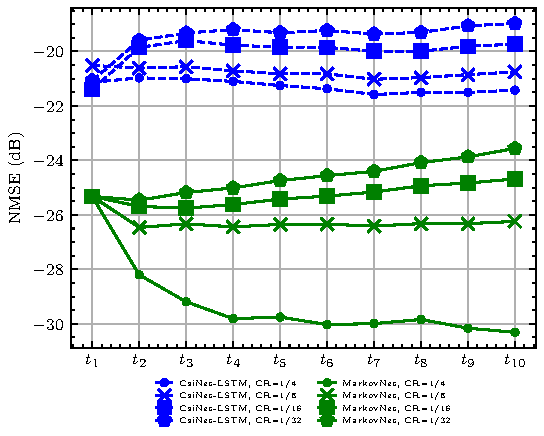
\includegraphics[width=\linewidth]{MarkovNet_truncated_Indoor_10slots.pdf}
		\caption{Indoor}
		\label{fig:diffnet_indoor} 
	\end{subfigure}
	\begin{subfigure}[t]{.45\textwidth}
		\centering
		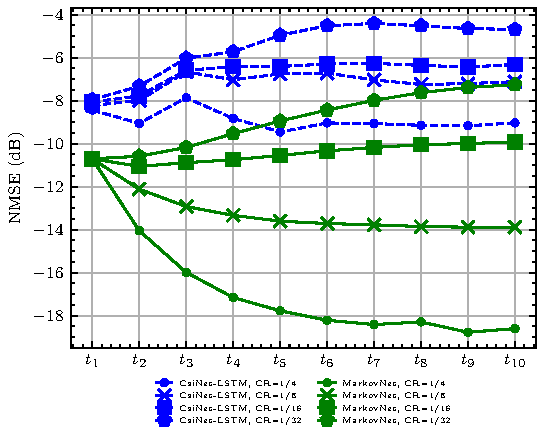
\includegraphics[width=\linewidth]{MarkovNet_truncated_Outdoor_10slots.pdf}
		\caption{Outdoor}
		\label{fig:diffnet_outdoor} 
	\end{subfigure}
	\caption{$\text{NMSE}$ comparison of MarkovNet and CsiNet-LSTM 
	at various compression ratios (CR).} 
	\label{fig:diffnet_result} \vspace*{-2mm}
\end{figure}  
Figure~\ref{fig:csi_image} shows a random sample from the test set, $\mathbf H$, and the estimates produced by CsiNet-LSTM and MarkovNet for a CR of $\frac 14$. This sample contains three ``peak'' magnitude regions. While both networks manage to capture the two larger samples, MarkovNet is able to recover the small peak magnitude region ({\color{darkgreen}green arrow}) which CsiNet-LSTM fails to produce ({\color{red}red arrow}).

\begin{figure}[htb] \centering 
	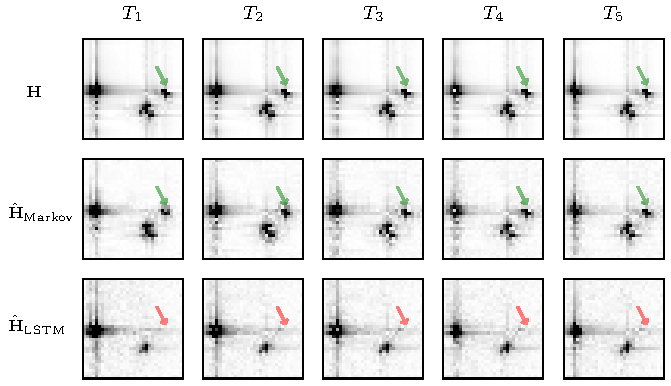
\includegraphics[width=0.9\linewidth]{batch0_csi_compare_cr512_annot.pdf}
	\caption{CSI ($\mathbf H$), MarkovNet estimates ($\hat{\mathbf H}_{\text{Markov}}$), and CsiNet-LSTM estimates ($\hat{\mathbf H}_{\text{LSTM}}$) across five timeslots ($T_1$ through $T_5$) on one outdoor channel sample from the test set,
using $\text{CR}=\frac 14$.} 
	\label{fig:csi_image} 
\end{figure}

To understand the effect of quantization on the network performance, we choose to use $\mu$-law companding and uniform quantization on the latent feedback elements. We begin by performing a logarithmic scaling on the feedback elements, $x$,
\begin{align}
	f(x) = \frac{\text{sign}(x)\ln\left(1 + \mu|x|\right)}{\ln\left(1 + \mu\right)} , \; 0 \leq |x| \leq 1. \label{eq:mu-forward}
\end{align}
After applying (\ref{eq:mu-forward}) to the signal, uniform quantization is applied to yield
\begin{align}
	\hat x = \Delta\left\lfloor\frac{f(x)}{\Delta}\right\rceil \label{eq:unif-quant}
\end{align}
where $\Delta = 2^{-(b-1)}$ for $b$-bit quantization. Finally, an inverse logarithmic scaling is applied to quantized signal,
\begin{align}
	F(\hat x) = \frac{\text{sign}(\hat x)\left(1 + \mu\right)^{|\hat x|} - 1}{\mu} , \; -1 \leq \hat x \leq 1. \label{eq:mu-backward}
\end{align}
In short, the described $\mu$-law quantization scheme involves applying (\ref{eq:mu-forward}), then (\ref{eq:unif-quant}), then (\ref{eq:mu-backward}) to each feedback element. Figures~\ref{fig:feedback_quant_indoor} and~\ref{fig:feedback_quant_outdoor} show the performance of MarkovNet and CsiNet-LSTM under $\mu$-law quantization where $\mu=255$.

In the Outdoor scenario, the performance of each network at each compression ratio does not change substantially for different numbers of quantization bits. In contrast, the performance for each network/compression ratio in the Indoor scenario drops appreciably for smaller quantization bits. We note that the performance of either network could potentially benefit from quantization during training, as all the results in Figures~\ref{fig:diffnet_indoor} and~\ref{fig:diffnet_outdoor} are trained with continuous feedback.

\begin{figure}[!hbtp] \centering 
	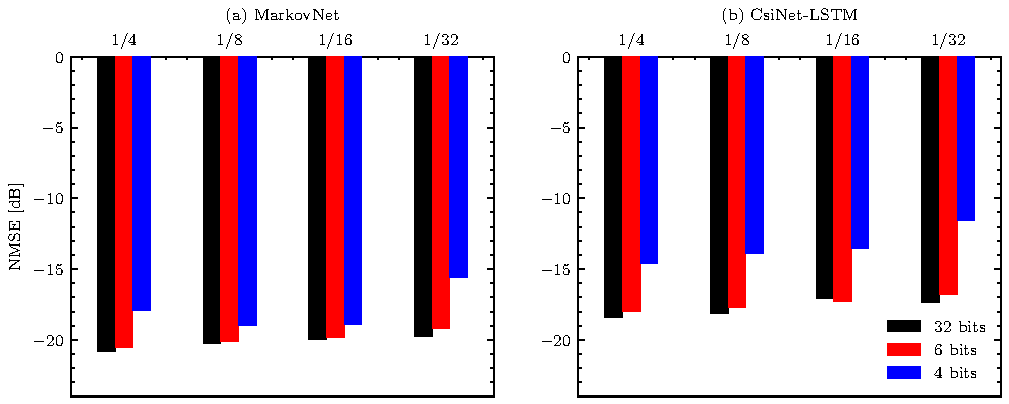
\includegraphics[width=\textwidth]{Indoor_feedback_quant.pdf}
    \caption{NMSE comparison of MarkovNet and CsiNet-LSTM for the Indoor scenario with feedback subject to $\mu$-law quantization using fixed step size, $\Delta=2^{-(b-1)}$, for $b$ bits.}
	\label{fig:feedback_quant_indoor} \vspace*{-2mm}
\end{figure}

\begin{figure}[!hbtp] \centering 
	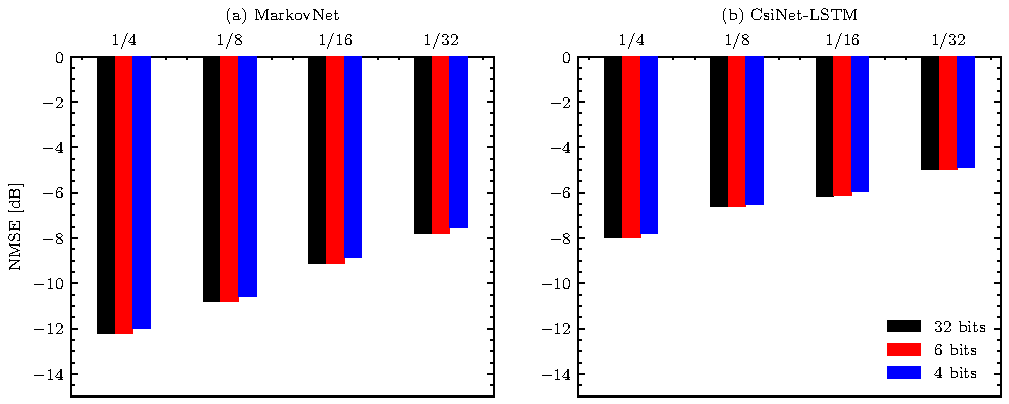
\includegraphics[width=\textwidth]{Outdoor_feedback_quant.pdf}
    \caption{NMSE comparison of MarkovNet and CsiNet-LSTM for the Outdoor scenario with feedback subject to $\mu$-law quantization using fixed step size, $\Delta=2^{-(b-1)}$, for $b$ bits.}
	\label{fig:feedback_quant_outdoor} \vspace*{-6mm}
\end{figure}